\documentclass[UTF8,a4paper,zihao=-4,fontset=mac]{ctexart}

\usepackage[left=2.55cm,right=2.55cm,top=2.55cm,bottom=2.45cm]{geometry}
\usepackage{graphicx}
\usepackage{booktabs}
\usepackage{tabularx}
\usepackage{longtable}
\usepackage{array}
\usepackage[table]{xcolor}
\usepackage{setspace}
\usepackage{enumitem}
\usepackage{float}
\usepackage{caption}
\usepackage{fancyhdr}
\usepackage{titlesec}
\usepackage{tikz}
\usetikzlibrary{arrows.meta,positioning,calc,shapes.geometric}
\usepackage{pifont}
\usepackage{hyperref}
\usepackage{bookmark}

\definecolor{PetGreen}{HTML}{174A3A}
\definecolor{PetGreenTwo}{HTML}{2E6A55}
\definecolor{PetOrange}{HTML}{D46D4C}
\definecolor{PetCream}{HTML}{F7F2E8}
\definecolor{PetPale}{HTML}{EAF2EE}
\definecolor{PetGray}{HTML}{65706B}
\definecolor{RuleGray}{HTML}{D6DED9}

\hypersetup{
  colorlinks=true,
  linkcolor=PetGreen,
  urlcolor=PetGreenTwo,
  citecolor=PetGreen,
  bookmarksnumbered=true,
  bookmarksopen=true,
  pdfauthor={琚昊，韩旭},
  pdftitle={PetLink 第三阶段第1周开发进展报告},
  pdfsubject={软件课程设计 I 阶段进展报告}
}

\setstretch{1.5}
\setlength{\parindent}{2em}
\setlength{\parskip}{0pt}
\setcounter{tocdepth}{2}
\setcounter{secnumdepth}{3}
\setlist[itemize]{leftmargin=2.2em,itemsep=0.2em,topsep=0.3em}
\setlist[enumerate]{leftmargin=2.4em,itemsep=0.2em,topsep=0.3em}

\titleformat{\section}{\zihao{3}\bfseries\color{PetGreen}}{\thesection}{0.75em}{}
\titleformat{\subsection}{\zihao{4}\bfseries\color{PetGreenTwo}}{\thesubsection}{0.7em}{}
\titleformat{\subsubsection}{\zihao{-4}\bfseries\color{PetGreen}}{\thesubsubsection}{0.6em}{}
\titlespacing*{\section}{0pt}{1.5em}{0.75em}
\titlespacing*{\subsection}{0pt}{1.15em}{0.5em}
\titlespacing*{\subsubsection}{0pt}{0.9em}{0.35em}

\captionsetup{font=small,labelfont=bf,labelsep=quad}
\captionsetup[table]{position=top,skip=6pt}
\captionsetup[figure]{position=bottom,skip=6pt}

\pagestyle{fancy}
\fancyhf{}
\fancyhead[L]{\zihao{5}\color{PetGray}PetLink 第三阶段第1周开发进展报告}
\fancyhead[R]{\zihao{5}\color{PetGray}软件课程设计 I}
\fancyfoot[C]{\zihao{5}\thepage}
\renewcommand{\headrulewidth}{0.4pt}
\renewcommand{\headrule}{\hbox to\headwidth{\color{RuleGray}\leaders\hrule height \headrulewidth\hfill}}
\setlength{\headheight}{24pt}
\setlength{\headsep}{12pt}

\newcolumntype{Y}{>{\raggedright\arraybackslash}X}
\newcolumntype{C}[1]{>{\centering\arraybackslash}p{#1}}
\newcolumntype{L}[1]{>{\raggedright\arraybackslash}p{#1}}
\newcommand{\pass}{\textcolor{PetGreen}{\ding{51}}}
\newcommand{\todo}{\textcolor{PetOrange}{\ding{115}}}
\newcommand{\code}[1]{\texttt{\small #1}}
\newcommand{\tablehead}{\rowcolor{PetGreen}\color{white}\bfseries}
\graphicspath{{assets/}}

\begin{document}
\pagenumbering{gobble}

% -------------------- 封面 --------------------
\begin{titlepage}
\thispagestyle{empty}
\begin{tikzpicture}[remember picture,overlay]
  \fill[PetCream] (current page.south west) rectangle (current page.north east);
  \fill[PetGreen] (current page.north west) rectangle ([yshift=-2.2cm]current page.north east);
  \fill[PetOrange] ([xshift=2.55cm,yshift=-2.2cm]current page.north west) rectangle ++(4.2cm,-0.13cm);
  \fill[PetGreen] (current page.south west) rectangle ([yshift=0.8cm]current page.south east);
  \node[anchor=west,text=white,font=\zihao{2}\bfseries]
    at ([xshift=2.55cm,yshift=-0.78cm]current page.north west) {软件课程设计 I};
  \node[anchor=west,text=white,font=\zihao{-4}]
    at ([xshift=2.55cm,yshift=-1.45cm]current page.north west) {阶段性开发成果汇报};
\end{tikzpicture}

\vspace*{2.1cm}
{\color{PetGreen}\zihao{1}\bfseries PetLink\par}
\vspace{0.25cm}
{\color{PetGreen}\zihao{2}\bfseries 流浪动物救助与领养服务平台\par}
\vspace{0.85cm}
{\color{PetOrange}\zihao{0}\bfseries 第三阶段第1周\par}
\vspace{0.2cm}
{\color{PetGreen}\zihao{1}\bfseries 开发进展报告\par}

\vspace{1.35cm}
\begin{center}
\begin{tikzpicture}
  \draw[PetPale,line width=12pt] (90:1.35) arc[start angle=90,end angle=-270,radius=1.35];
  \draw[PetGreen,line width=12pt,line cap=round] (90:1.35) arc[start angle=90,end angle=-255.6,radius=1.35];
  \node[align=center,text=PetGreen] at (0,0) {\zihao{1}\bfseries 96\%\\[-0.2em]\zihao{5}\bfseries 总体进度};
\end{tikzpicture}
\end{center}

\vspace{0.7cm}
\renewcommand{\arraystretch}{1.55}
\begin{center}
\begin{tabular}{L{3.2cm}L{8.5cm}}
课题名称 & PetLink 流浪动物救助与领养服务平台 \\
报告类型 & 第三阶段第1周开发进展报告 \\
组长 & 琚昊（学号：924106840421） \\
成员 & 韩旭（学号：924106840417） \\
进度统计日期 & 2026 年 9 月 6 日 \\
计划完成日期 & 2026 年 9 月 13 日前 \\
\end{tabular}
\end{center}
\end{titlepage}

% -------------------- 目录 --------------------
\pagestyle{empty}
\thispagestyle{empty}
\pdfbookmark[0]{目录}{toc}
\begin{center}
  {\zihao{2}\bfseries\color{PetGreen}目\quad 录}
\end{center}
\vspace{0.8cm}
\makeatletter\@starttoc{toc}\makeatother
\clearpage

\pagenumbering{arabic}
\setcounter{page}{1}
\pagestyle{fancy}

\section{本周进展结论}

截至 2026 年 9 月 6 日，PetLink 已完成计划内 M01--M08 全部功能开发，完成 PC 端、Mobile H5 端与 Spring Boot 后端的联通，并在公网服务器形成可访问的部署版本。按工作分解结构加权计算，第三阶段总体完成度为 \textbf{96\%}；其中，\textbf{计划内功能开发完成度为 100\%}，剩余 4\% 为独立 Chrome/Edge 兼容复核、HBuilderX 与 Android/iOS 真机验证，以及提交前最终回归和归档。

本周重新执行的全量自动化门禁全部通过：后端 JUnit \textbf{297/297}、PC Node \textbf{36/36}、Mobile Node \textbf{18/18}；跨平台三角色核心业务链路 \textbf{40/40} 通过。计划内 52 条 RTM 原子条目和 72 个 Frozen REST API 均已建立实现与测试证据。数据库结构为 16 张物理表、52 个 CHECK 约束、26 个外键和 17 个唯一约束。主要结果汇总见表~\ref{tab:headline}。

\begin{table}[H]
\centering
\caption{第三阶段第1周核心进展指标}
\label{tab:headline}
\rowcolors{2}{PetPale}{white}
\begin{tabularx}{\textwidth}{L{3.8cm}C{2.8cm}Y}
\toprule
\rowcolor{PetGreen}\color{white}\bfseries 指标 & \color{white}\bfseries 当前结果 & \color{white}\bfseries 判定 \\
\midrule
第三阶段总体进度 & 96\% & 进入兼容性复核和最终归档阶段 \\
计划内功能开发 & 100\% & M01--M08 全部实现并冻结 \\
当前全量自动化门禁 & 351/351 & 后端 297、PC 36、Mobile 18，全部通过 \\
跨平台主业务联通 & 40/40 & USER、RESCUER、ADMIN 共享同一业务数据 \\
需求与接口追踪 & 52/52；72/72 & RTM 条目和 Frozen API 均有实现与测试证据 \\
数据库结构 & 16 张表 & 52 CHECK、26 FK、17 UNIQUE \\
部署状态 & 已上线 & PC、Mobile 与 API 通过 8081 端口提供服务 \\
\bottomrule
\end{tabularx}
\end{table}

基于上述结果，项目组判断：\textbf{能够在第三阶段第2周，即 2026 年 9 月 13 日前完成全部开发和测试工作。}当前不存在阻断主业务闭环的功能缺陷，后续任务范围清晰、可复现，并已预留缺陷修复缓冲时间。

\clearpage
\section{计划依据与本周阶段定位}

\subsection{计划书对编码测试阶段的要求}

《PetLink 详细设计说明书 V1.0 Frozen》已经完成需求、架构、数据库、M01--M08 模块、核心用例、事务并发、文件管理和 UI 设计的冻结。计划书第 10.3 节给出的实施顺序是：先建立 Spring Boot 2.7.18、JDK 17、MyBatis-Plus 与 MySQL 工程骨架；先实现 M01 认证和全局安全，再完成 M02--M04 救助主链，随后完成 M05--M07 领养、回访和公告，最后完成 M08；同时围绕锁顺序、事务、幂等和文件补偿编写测试，把 PC 与 UniApp 原型迁移为真实数据驱动页面，并依据结果回填 RTM。

第三阶段第1周的实际工作已经覆盖以上全部实施步骤，并进一步完成公众首页、角色工作台、前端中文化、UI/UX 收口、后端查询性能治理、部署与回滚准备。因此，本周不再属于单一模块编码阶段，而是“计划内功能冻结完成、产品化收口和整体验收并行”的阶段。

\subsection{系统范围与技术架构}

PetLink 采用 PC 与 Mobile 双前端共享 REST API 的前后端分离架构。Spring Security 与 JWT 负责身份认证，Controller 负责协议适配，Service 承担业务规则、事务和并发控制，MyBatis-Plus Mapper 访问 MySQL，文件服务统一处理临时上传、正式绑定与清理。系统架构如图~\ref{fig:architecture} 所示。

\begin{figure}[H]
\centering
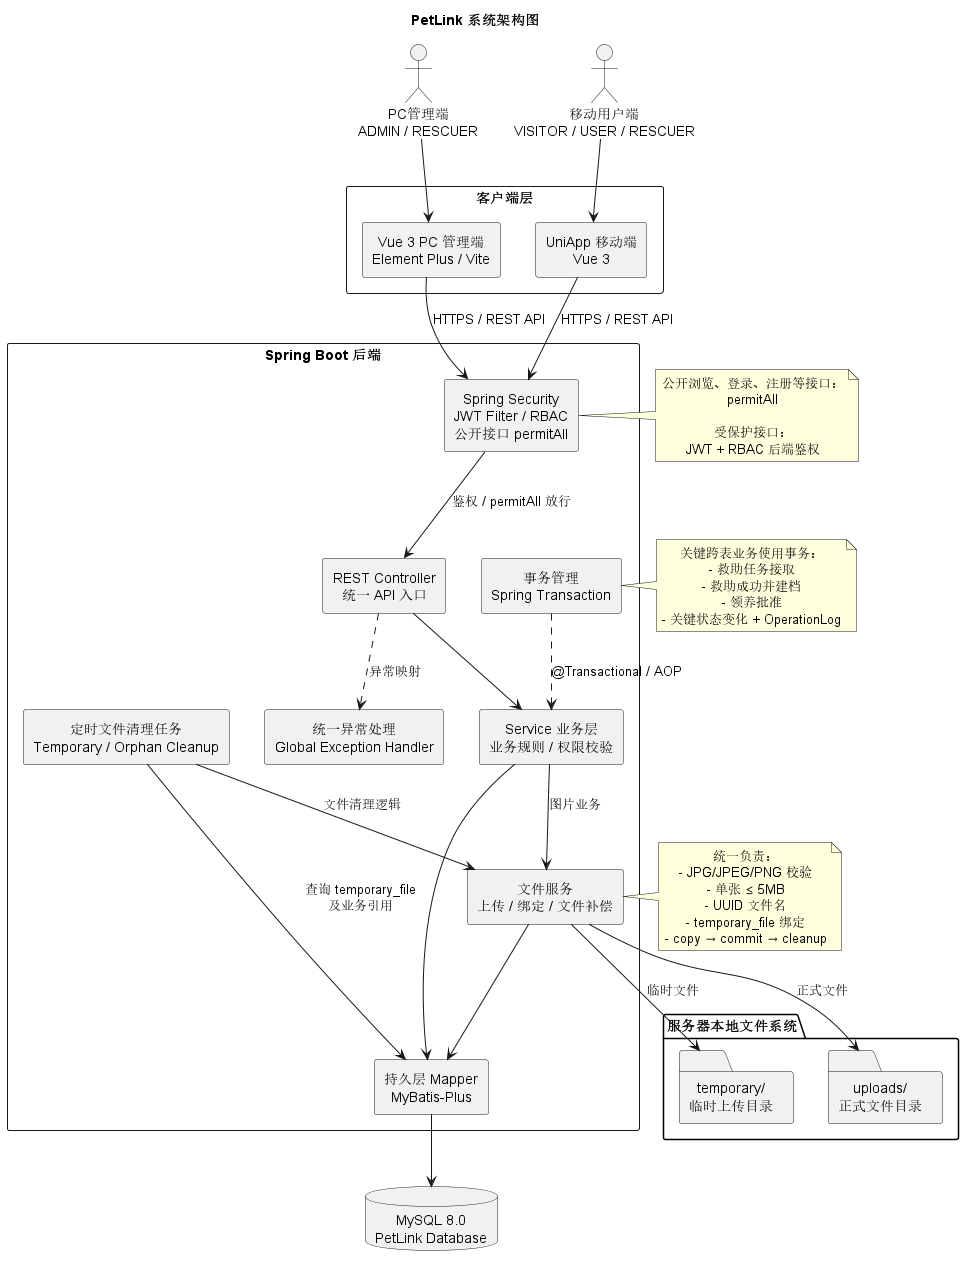
\includegraphics[width=0.92\textwidth]{system-architecture.png}
\caption{PetLink 双端共享后端的系统架构}
\label{fig:architecture}
\end{figure}

该架构保证两类终端不是相互独立的演示系统：普通用户在 Mobile 发布线索或申请领养后，管理员能够在 PC 审核；管理员审核通过后，救助人员能在 PC 或 Mobile 查看待接任务并继续处理，最终状态仍回写同一数据库。

\section{开发进度量化}

\subsection{总体完成度计算方法}

为使百分比可解释，本报告按需求基线、后端与数据库、PC、Mobile、质量保证、部署、独立环境兼容、最终回归归档八类交付物分配权重。完成度按“权重 $\times$ 当前完成比例”求和，结果为 96\%，明细见表~\ref{tab:weighted-progress}。该口径区分“功能是否开发完成”和“课程交付是否全部收尾”，避免把尚未进行的真机签字误写为已完成。

\begin{table}[H]
\centering
\caption{第三阶段工作分解与加权完成度}
\label{tab:weighted-progress}
\rowcolors{2}{PetPale}{white}
\begin{tabularx}{\textwidth}{Y C{1.8cm} C{2.2cm} C{2.2cm}}
\toprule
\rowcolor{PetGreen}\color{white}\bfseries 工作项 & \color{white}\bfseries 权重 & \color{white}\bfseries 完成比例 & \color{white}\bfseries 进度贡献 \\
\midrule
需求、设计与 RTM 基线 & 8\% & 100\% & 8.0\% \\
后端服务与数据库 & 24\% & 100\% & 24.0\% \\
PC 公众站与工作台 & 17\% & 100\% & 17.0\% \\
Mobile H5 应用 & 16\% & 100\% & 16.0\% \\
自动化、E2E、安全与性能测试 & 22\% & 100\% & 22.0\% \\
服务器部署、备份和回滚准备 & 7\% & 100\% & 7.0\% \\
独立浏览器、HBuilderX 与真机复核 & 4\% & 25\% & 1.0\% \\
最终回归、证据归档与提交包核验 & 2\% & 50\% & 1.0\% \\
\midrule
\textbf{合计} & \textbf{100\%} & -- & \textbf{96.0\%} \\
\bottomrule
\end{tabularx}
\end{table}

图~\ref{fig:progress-bars} 将完成度按开发、自动化测试、部署和交付收尾四个层次展示。功能开发和自动化测试已经达到 100\%，进度缺口集中在独立环境的人工复核，而不是核心代码缺失。

\begin{figure}[H]
\centering
\begin{tikzpicture}[x=0.065\textwidth,y=0.75cm]
  \def\bar#1#2#3{
    \node[anchor=east,text=PetGray,font=\small] at (-0.18,#1) {#2};
    \fill[PetPale,rounded corners=2pt] (0,#1-0.18) rectangle (10,#1+0.18);
    \fill[PetGreen,rounded corners=2pt] (0,#1-0.18) rectangle (#3/10,#1+0.18);
    \node[anchor=west,font=\small\bfseries,text=PetGreen] at (10.15,#1) {#3\%};
  }
  \bar{3}{功能开发}{100}
  \bar{2}{自动化与主链测试}{100}
  \bar{1}{部署与回滚准备}{100}
  \bar{0}{第三阶段总体}{96}
\end{tikzpicture}
\caption{第三阶段第1周关键工作完成度}
\label{fig:progress-bars}
\end{figure}

\clearpage
\section{已经完成的开发工作与成果}

\subsection{M01--M08 计划内模块全部完成}

功能模块不是围绕数据表做简单增删查改，而是围绕真实业务状态和角色协作组织。图~\ref{fig:modules} 展示了 M01--M08 的划分，表~\ref{tab:modules} 则给出每个模块已经形成的可验收结果。

\begin{figure}[H]
\centering
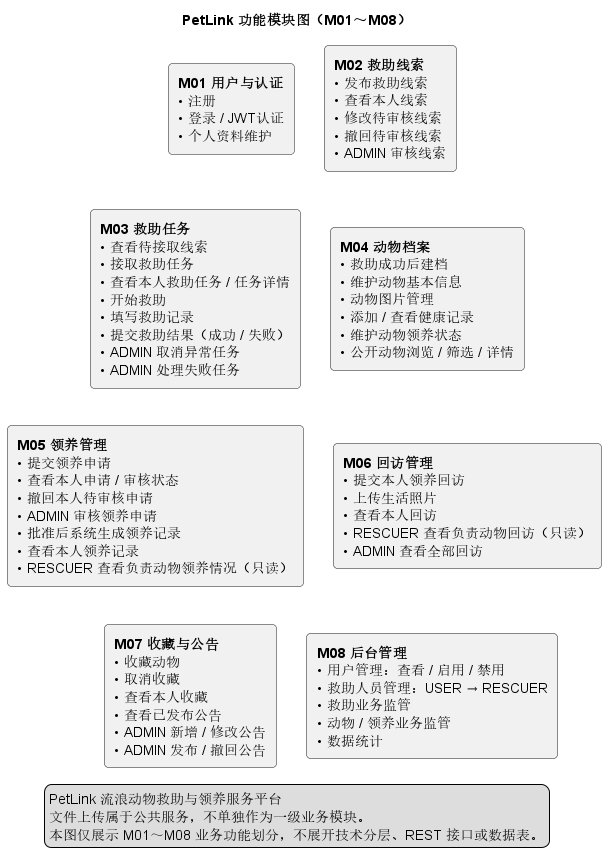
\includegraphics[width=0.92\textwidth]{functional-modules.png}
\caption{PetLink M01--M08 功能模块结构}
\label{fig:modules}
\end{figure}

\begin{longtable}{L{1.1cm}L{3.1cm}L{8.7cm}C{1.3cm}}
\caption{M01--M08 已完成开发成果}\label{tab:modules}\\
\toprule
\rowcolor{PetGreen}\color{white}\bfseries 模块 & \color{white}\bfseries 业务范围 & \color{white}\bfseries 已完成成果 & \color{white}\bfseries 状态 \\
\midrule
\endfirsthead
\multicolumn{4}{l}{\zihao{5}\color{PetGray}表~\thetable\ （续）}\\
\toprule
\rowcolor{PetGreen}\color{white}\bfseries 模块 & \color{white}\bfseries 业务范围 & \color{white}\bfseries 已完成成果 & \color{white}\bfseries 状态 \\
\midrule
\endhead
\bottomrule
\endfoot
M01 & 用户与认证 & 注册、登录、JWT 鉴权、当前用户资料、账号状态和角色即时刷新；密码 BCrypt 存储，账号规范化与密码长度边界已测试。 & \pass \\
\rowcolor{PetPale}
M02 & 救助线索 & 线索发布、图片绑定、查看、修改、撤回、审核通过/驳回；短期幂等键、请求指纹和操作日志已实现。 & \pass \\
M03 & 救助任务 & 待接取、原子接单、开始、过程记录、成功/失败、管理员异常处置；接单并发和活动任务唯一性已受保护。 & \pass \\
\rowcolor{PetPale}
M04 & 动物档案 & 救助成功自动建档、图片与健康记录、负责动物查询、治疗/观察/开放领养/暂停领养状态流转。 & \pass \\
M05 & 领养业务 & 领养申请、撤回、管理员审核、成功领养记录、同动物其他申请自动失效；批准事务采用固定锁顺序。 & \pass \\
\rowcolor{PetPale}
M06 & 领养回访 & 回访提交、历史查询、图片、普通用户/救助人员/管理员可见性；永久幂等和并发重放恢复已完成。 & \pass \\
M07 & 收藏与公告 & 收藏/取消收藏幂等，公告草稿、编辑、发布、撤回、公开查看；新增带版本校验的逻辑删除与检索。 & \pass \\
\rowcolor{PetPale}
M08 & 后台管理 & 用户详情、启禁用、救助人员角色变更、逻辑删除、业务监管、概览与日期趋势统计；管理员保护规则已完成。 & \pass \\
\end{longtable}

\subsection{双平台三角色已经形成完整业务闭环}

目前系统已经打通 USER、RESCUER、ADMIN 三类用户在 PC 和 Mobile 两个平台之间的数据流。主流程不是页面级的独立演示，而是同一组数据库记录依次发生状态变化，如图~\ref{fig:closed-loop} 所示。

\begin{figure}[H]
\centering
\begin{tikzpicture}[
  node distance=0.55cm and 0.35cm,
  flowbox/.style={rounded corners=3pt,draw=PetGreen,line width=0.7pt,fill=PetPale,
    minimum height=1.05cm,text width=2.05cm,align=center,font=\small\bfseries},
  actor/.style={font=\scriptsize,text=PetOrange},
  arr/.style={-{Stealth[length=2.5mm]},line width=0.8pt,draw=PetGreenTwo}
]
\node[flowbox] (clue) {发现并发布\\救助线索};
\node[flowbox,right=of clue] (audit) {管理员\\审核线索};
\node[flowbox,right=of audit] (rescue) {救助人员\\接取并救助};
\node[flowbox,right=of rescue] (animal) {成功后自动\\建立动物档案};
\node[flowbox,below=1.2cm of animal] (open) {档案状态流转\\开放领养};
\node[flowbox,left=of open] (apply) {用户提交\\领养申请};
\node[flowbox,left=of apply] (approve) {管理员审核\\生成领养记录};
\node[flowbox,left=of approve] (follow) {领养人提交\\后续回访};
\draw[arr] (clue) -- (audit);
\draw[arr] (audit) -- (rescue);
\draw[arr] (rescue) -- (animal);
\draw[arr] (animal) -- (open);
\draw[arr] (open) -- (apply);
\draw[arr] (apply) -- (approve);
\draw[arr] (approve) -- (follow);
\node[actor,above=0.12cm of clue] {Mobile USER/RESCUER};
\node[actor,above=0.12cm of audit] {PC ADMIN};
\node[actor,above=0.12cm of rescue] {PC / Mobile RESCUER};
\node[actor,below=0.12cm of follow] {Mobile USER};
\end{tikzpicture}
\caption{线索到回访的双平台三角色业务闭环}
\label{fig:closed-loop}
\end{figure}

真实跨平台 E2E 已验证以下关键联动：Mobile 注册并发布线索，PC 管理员审核后两个前端的救助人员都能看到待接取信息；Mobile 接取后 PC 待接列表同步移除；PC 开始任务，Mobile 追加救助记录，PC 提交成功并建档；用户收藏并申请领养，管理员批准后生成领养记录；用户提交回访，救助人员可查看；管理员禁用账号后旧令牌立即失效。全链路共 40 项检查，全部通过。

\subsection{产品化与用户体验改进}

在 Frozen 计划内功能完成后，本周还完成了影响实际使用体验的产品化工作：PC 端增加公众首页、领养浏览、公告、参与指南和注册入口；管理员与救助人员使用角色工作台；Mobile 根据角色动态展示入口，并在页面显示时刷新任务队列。两端用户可见状态、角色、物种、性别和错误信息均已中文化。

前端已统一视觉令牌、品牌标识、按钮高度、焦点态、对话框位置、错误反馈和语义 SVG 图标；列表请求增加竞态保护，较慢的旧请求不会覆盖最新筛选结果。登录失败会在页面内给出可理解的中文提示，断网初始加载不再造成未处理异常。公众首页使用按需加载和路由懒加载，首屏关键传输量由约 744 KB 降至约 154 KB，减少约 79\%。

\section{复杂业务逻辑与具体设计落实}

\subsection{功能需求与设计实现对应}

表~\ref{tab:requirement-design} 说明主要功能需求如何落实到状态机、事务、数据库约束和测试。由此可见，本项目的业务复杂度来自跨角色协作和一致性控制，而不是只完成界面的增删查改。

\begin{longtable}{L{2.5cm}L{3.1cm}L{5.3cm}L{3.0cm}}
\caption{核心功能需求与设计实现对应关系}\label{tab:requirement-design}\\
\toprule
\rowcolor{PetGreen}\color{white}\bfseries 功能点 & \color{white}\bfseries 需求规定 & \color{white}\bfseries 具体设计实现 & \color{white}\bfseries 验证结果 \\
\midrule
\endfirsthead
\multicolumn{4}{l}{\zihao{5}\color{PetGray}表~\thetable\ （续）}\\
\toprule
\rowcolor{PetGreen}\color{white}\bfseries 功能点 & \color{white}\bfseries 需求规定 & \color{white}\bfseries 具体设计实现 & \color{white}\bfseries 验证结果 \\
\midrule
\endhead
\bottomrule
\endfoot
线索发布 & 至少一张图片；地点、时间、描述和联系方式有效；重复点击不能产生重复线索 & 10 分钟短期幂等键，DTO 规范化后计算 SHA-256 指纹，执行 UNUSED--PROCESSING--SUCCEEDED 原子流转 & 重放返回同一结果；图片与日志同事务 \\
\rowcolor{PetPale}
线索审核 & 仅管理员处理待审核线索；驳回必须填写原因 & Service 校验角色与 PENDING\_REVIEW 状态，审核操作写 reviewer\_id、reviewed\_at 和 OperationLog & 通过后进入 WAITING\_ACCEPT，驳回信息完整 \\
救助接单 & 同一线索只能被一名救助人员接取 & 条件更新 Clue 后创建 Task；active\_clue\_id 生成列加唯一约束作为并发兜底；失败整体回滚 & 并发接单只允许一个成功 \\
\rowcolor{PetPale}
救助成功建档 & 成功任务必须至少生成一个动物档案，过程事实不可丢失 & 固定 Task--Clue 锁顺序，事务内创建 Animal、可选 HealthRecord、图片和日志，并关闭线索 & 跨表结果一致，任一失败整体回滚 \\
领养批准 & 动物只能成功领养一次，其他待审核申请自动失效 & 固定 Animal--目标 Application--其他 Application 锁顺序；唯一 AdoptionRecord；更新 Animal 为 ADOPTED & 并发批准、乐观锁和自动失效均通过 \\
\rowcolor{PetPale}
领养回访 & 内容、健康情况或图片至少提供一项；重复提交不能重复落库 & submitter\_id 与 idempotency\_key 唯一，先插回访再绑定图片；并发冲突恢复为首次记录 & 永久幂等与 0--9 张图片边界通过 \\
账号与权限 & 角色和启禁用状态应即时生效，前端隐藏不能代替后端校验 & 每次受保护请求从数据库刷新当前角色和状态；Controller 和 Service 双重授权；敏感资源越权返回 403/404 & 禁用、恢复、升降级和越权测试通过 \\
\end{longtable}

救助成功建档是系统中最关键的跨表事务之一，其原子步骤如图~\ref{fig:rescue-sequence} 所示。任务、线索、动物、健康记录、图片和操作日志在一个受控事务内推进，避免出现“任务成功但没有动物档案”或“数据库已提交但图片未绑定”的半完成状态。

\begin{figure}[H]
\centering
\begin{tikzpicture}[
  txn/.style={rounded corners=3pt,draw=PetGreen,line width=0.7pt,fill=PetPale,
    minimum height=1.25cm,text width=2.18cm,align=center,font=\small\bfseries},
  arr/.style={-{Stealth[length=2.5mm]},line width=0.8pt,draw=PetGreenTwo}
]
\node[txn] (lock) {校验负责人\\锁定 Task 与 Clue};
\node[txn,right=0.28cm of lock] (task) {Task 更新为 SUCCESS\\写完成时间};
\node[txn,right=0.28cm of task] (animal) {创建 Animal\\健康记录与图片};
\node[txn,right=0.28cm of animal] (clue) {Clue 更新为 CLOSED\\写操作日志};
\node[txn,right=0.28cm of clue] (commit) {统一提交事务\\返回完整结果};
\draw[arr] (lock) -- (task);
\draw[arr] (task) -- (animal);
\draw[arr] (animal) -- (clue);
\draw[arr] (clue) -- (commit);
\node[below=0.48cm of animal,align=center,text=PetOrange,font=\small]
  {任一步骤失败：数据库整体回滚；仅清理本事务新建的正式文件副本};
\end{tikzpicture}
\caption{救助成功并建立动物档案的原子事务步骤}
\label{fig:rescue-sequence}
\end{figure}

\subsection{异常、安全与可追溯性}

系统已覆盖 JWT 失效、角色越权、资源归属、非法状态迁移、版本冲突、幂等冲突、文件回滚、危险路径、清理任务单行故障隔离等异常分支。关键状态变化与管理操作写入 append-only 的 \code{operation\_log}，并与业务事务同时提交；请求携带关联 ID，便于把前端报错、接口日志和后端处理串联起来。

HTTP 层统一返回 400、401、403、404、409、413 和 500 等状态与业务错误码。普通用户不会看到数据库异常或服务端堆栈。线索、任务、动物、领养、回访、公告和用户列表采用服务端分页、搜索与筛选，避免数据增长后一次性加载全部记录。

\section{数据库设计与资源命名复核}

\subsection{数据库是否满足业务场景}

数据库采用 MySQL 8.0 和 UTF-8 字符集，共 16 张物理表，其中 15 张为核心业务表，\code{temporary\_file} 为共享技术支撑表。实体覆盖用户、线索、任务、救助记录、动物、健康记录、领养申请、领养记录、回访、收藏、公告、操作日志和图片关系，能够完整保存业务事实，而不是只保存最终状态。

\begin{longtable}{L{3.0cm}L{5.2cm}L{5.7cm}}
\caption{必要业务数据的存储覆盖复核}\label{tab:data-coverage}\\
\toprule
\rowcolor{PetGreen}\color{white}\bfseries 业务场景 & \color{white}\bfseries 必要数据 & \color{white}\bfseries 当前存储设计 \\
\midrule
\endfirsthead
\multicolumn{3}{l}{\zihao{5}\color{PetGray}表~\thetable\ （续）}\\
\toprule
\rowcolor{PetGreen}\color{white}\bfseries 业务场景 & \color{white}\bfseries 必要数据 & \color{white}\bfseries 当前存储设计 \\
\midrule
\endhead
\bottomrule
\endfoot
线索审核 & 发布人、审核人、时间、结论、驳回原因 & publisher\_id、reviewer\_id、reviewed\_at、status、reject\_reason \\
\rowcolor{PetPale}
救助执行 & 接单人、开始/结束时间、过程记录、失败或取消原因 & rescuer\_id、started\_at、finished\_at、rescue\_record、failure/cancel\_reason \\
动物照护 & 来源任务、状态、健康情况、图片顺序和版本 & rescue\_task\_id、status、health\_record、animal\_image.sort\_order、version \\
\rowcolor{PetPale}
领养审核 & 申请人、动物、审核人、审核时间、最终领养事实 & adoption\_application 与唯一 adoption\_record，保存 reviewer\_id、reviewed\_at \\
领养回访 & 提交人、内容、健康情况、图片和幂等标识 & follow\_up\_record、follow\_up\_image、idempotency\_key \\
\rowcolor{PetPale}
审计与文件 & 状态前后值、原因、操作人；临时/正式文件状态 & operation\_log；temporary\_file 的 token、路径、owner、status \\
\end{longtable}

数据库约束形成第二层一致性防线：52 个 CHECK 约束限制枚举、必填文本、时间和状态关联；26 个外键保证实体关系；17 个唯一约束防止重复领养、重复收藏、重复图片顺序和重复幂等记录。业务状态迁移仍由 Service 层判断，数据库约束不替代业务逻辑。

\subsection{资源命名规范}

本周对设计和实现中的命名进行了统一复核。数据库表和字段采用蛇形命名法，主外键统一使用 \code{id} 与 \code{xxx\_id}，时间字段使用 \code{created\_at}、\code{updated\_at}、\code{reviewed\_at} 等后缀；外键、唯一和检查约束使用 \code{fk\_}、\code{uk\_}、\code{chk\_} 前缀。Java 类型使用 PascalCase，方法和变量使用 camelCase；REST 资源使用复数名词和连字符，例如 \code{/api/rescue-clues}、\code{/api/rescue-tasks} 和 \code{/api/adoption-applications}。前端路由名称与业务页面一致，避免使用无含义缩写。

该规范已经同步到 SQL、Mapper、Service、Controller、前端 API Client 和文档，减少大小写漂移、同一资源多种命名以及字段含义不清等问题。新增逻辑删除和角色变更仍沿用既有命名体系，没有另建与历史业务冲突的事实源。

\section{前端与 UI 设计完成情况}

\subsection{UI 设计原则已经落实}

冻结设计确定了“城市动物救助档案 + 温暖领养社区”的视觉方向。Mobile 突出动物图片、救助状态和行动入口，PC 突出审核队列、动物档案、监管和统计。图~\ref{fig:mobile-ui} 与图~\ref{fig:pc-ui} 均为 2026 年 9 月 6 日从 PetLink 公网部署版本直接截取的实际运行页面，能够证明设计稿已经转化为真实数据驱动、中文化且可交互的产品界面。

\begin{figure}[H]
\centering
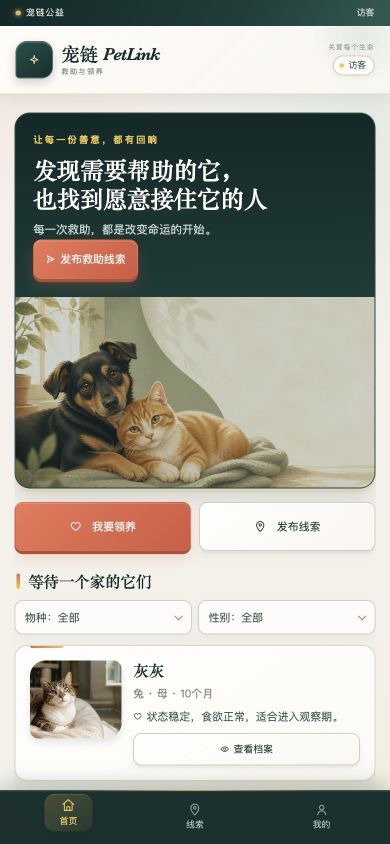
\includegraphics[width=0.43\textwidth]{actual-mobile-home.png}
\caption{公网部署版本 Mobile H5 首页实拍}
\label{fig:mobile-ui}
\end{figure}

Mobile 端共注册 29 个页面路由，全部在页面显示时执行角色/会话守卫。底部导航和业务入口随角色变化，普通用户不能通过直接输入路由进入救助人员页面；任务页每次显示时刷新“待接取”和“我的任务”，解决跨端审核后列表不同步的问题。

\begin{figure}[H]
\centering
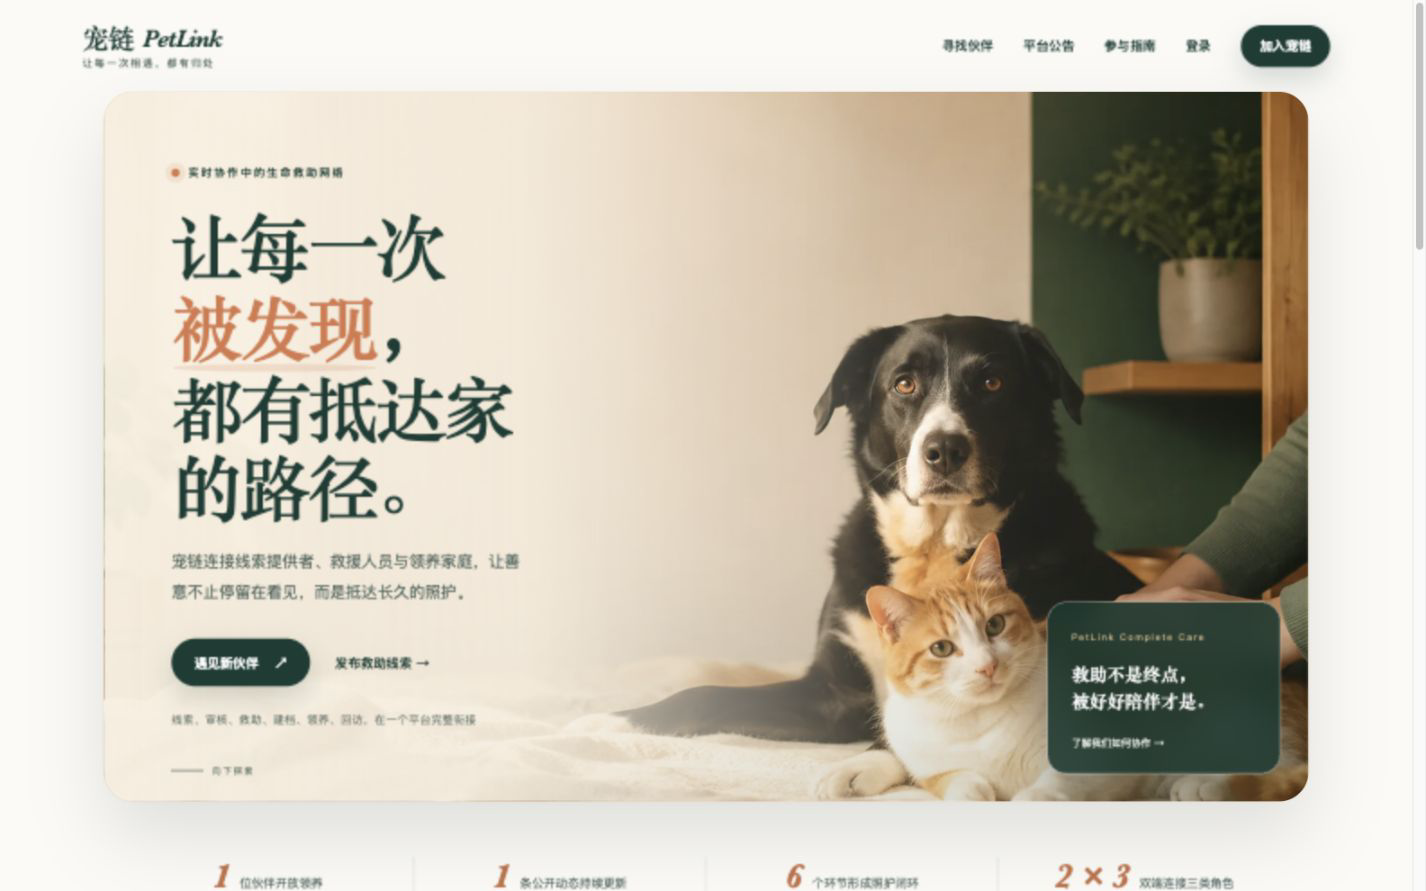
\includegraphics[width=0.92\textwidth]{actual-pc-home.png}
\caption{公网部署版本 PC 公众首页实拍}
\label{fig:pc-ui}
\end{figure}

PC 端已实现 10 个工作台页面及登录入口，并补充公众首页、寻找伙伴、动物详情、公告、参与指南和注册资源。工作台依据角色显示线索审核、任务、动物、领养、回访、公告、用户与统计入口；弹窗居中且限制高度，危险操作要求原因或二次确认，列表支持服务端筛选和分页。

\subsection{Web 资源与 UI 覆盖}

为落实“每个 Web 资源都有对应 UI”的要求，表~\ref{tab:ui-coverage} 按资源域核对了路由、角色、交互和状态展示。详细设计中的图 9-1 至图 9-10 已覆盖 29 个 Mobile 页面/状态视图和 PC 管理端主要页面；实现阶段继续以相同资源名称建立真实 Vue 页面。

\begin{longtable}{L{2.4cm}L{3.7cm}L{4.0cm}L{3.8cm}}
\caption{Web 资源与 UI 实现覆盖}\label{tab:ui-coverage}\\
\toprule
\rowcolor{PetGreen}\color{white}\bfseries 资源域 & \color{white}\bfseries PC UI & \color{white}\bfseries Mobile UI & \color{white}\bfseries 已实现交互 \\
\midrule
\endfirsthead
\multicolumn{4}{l}{\zihao{5}\color{PetGray}表~\thetable\ （续）}\\
\toprule
\rowcolor{PetGreen}\color{white}\bfseries 资源域 & \color{white}\bfseries PC UI & \color{white}\bfseries Mobile UI & \color{white}\bfseries 已实现交互 \\
\midrule
\endhead
\bottomrule
\endfoot
公众与认证 & 首页、寻找伙伴、公告、指南、注册、登录 & 首页、动物列表、登录、注册、个人资料 & 响应式导航、会话校验、中文错误反馈 \\
\rowcolor{PetPale}
救助线索 & 线索审核列表、详情和审核弹窗 & 发布、我的线索、编辑、线索详情 & 图片上传、幂等提交、状态标签、审核原因 \\
救助任务 & 待接取/我的任务、监管列表与详情 & 待接线索、待开始、执行中、记录、提交结果 & 跨端刷新、合法动作显示、失败/取消处理 \\
\rowcolor{PetPale}
动物档案 & 动物列表、详情、图片、健康和状态操作 & 负责动物、动物维护、动物详情 & 建档、健康记录、开放/暂停领养、版本冲突提示 \\
领养业务 & 申请审核与领养记录监管 & 申请表、申请详情、我的申请、领养记录 & 审核批准/拒绝、撤回、自动失效展示 \\
\rowcolor{PetPale}
回访收藏公告 & 回访监管、公告管理 & 回访提交/历史/详情、收藏、公告列表/详情 & 幂等、图片、发布/撤回、搜索和逻辑删除 \\
用户与统计 & 用户管理、角色变更、启禁用、总览和趋势 & 个人资料与编辑 & 权限即时生效、日期范围校验、状态分布和趋势图 \\
\end{longtable}

公众页面进一步使用真实动物数据和服务端公开查询接口。图~\ref{fig:adopt-ui} 展示了公网部署版本的“寻找伙伴”页面：筛选器、动物状态、基础档案和详情入口均已绑定后端数据。首页主视觉采用轻量 WebP，并配置明确宽高、懒加载、异步解码和减少动态效果偏好，兼顾视觉质量、加载性能与可访问性。

\begin{figure}[H]
\centering
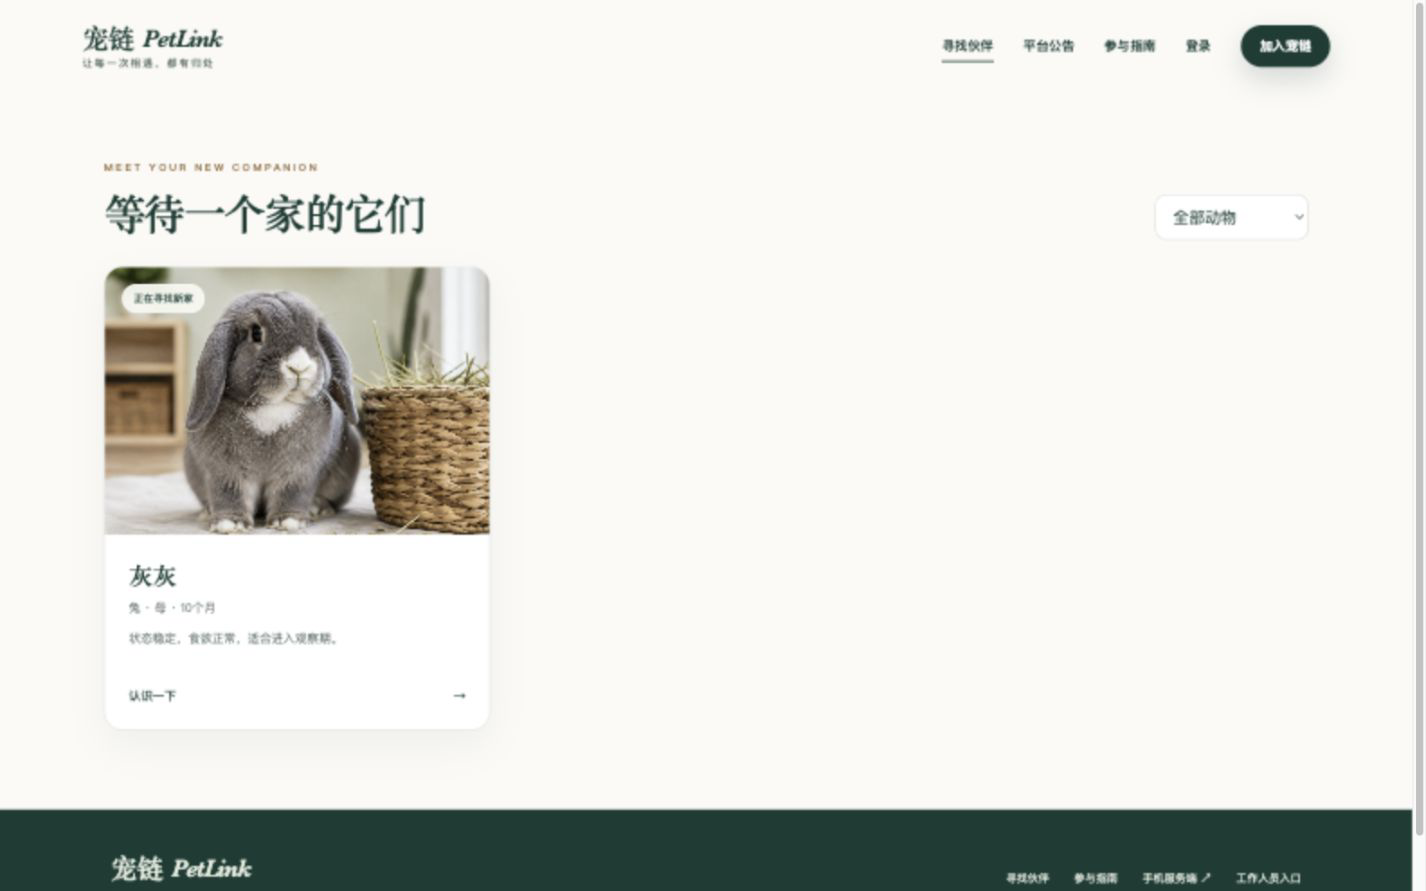
\includegraphics[width=0.92\textwidth]{actual-pc-adopt.png}
\caption{公网部署版本 PC“寻找伙伴”页面实拍}
\label{fig:adopt-ui}
\end{figure}

\section{测试、性能与质量成果}

\subsection{本周最新全量验证}

2026 年 9 月 6 日在当前工作树重新执行 \code{scripts/verify-all.sh}，后端、数据库静态门禁、PC、Mobile、前端契约和交付包哈希均通过。图~\ref{fig:test-result} 与表~\ref{tab:test-result} 汇总最新结果。

\begin{figure}[H]
\centering
\begin{tikzpicture}[x=0.018\textwidth,y=0.83cm]
  \def\testbar#1#2#3{
    \node[anchor=east,text=PetGray,font=\small] at (-2.2,#1) {#2};
    \fill[PetPale,rounded corners=2pt] (0,#1-0.2) rectangle (35,#1+0.2);
    \fill[PetGreen,rounded corners=2pt] (0,#1-0.2) rectangle (35,#1+0.2);
    \node[anchor=west,font=\small\bfseries,text=PetGreen] at (36,#1) {#3};
  }
  \testbar{3}{后端 JUnit}{297/297}
  \testbar{2}{PC Node}{36/36}
  \testbar{1}{Mobile Node}{18/18}
  \testbar{0}{跨平台 E2E}{40/40}
\end{tikzpicture}
\caption{当前主要自动化与跨平台测试通过情况}
\label{fig:test-result}
\end{figure}

\begin{table}[H]
\centering
\caption{测试与质量门禁结果}
\label{tab:test-result}
\rowcolors{2}{PetPale}{white}
\begin{tabularx}{\textwidth}{L{3.3cm}C{2.4cm}Y}
\toprule
\rowcolor{PetGreen}\color{white}\bfseries 验证层级 & \color{white}\bfseries 结果 & \color{white}\bfseries 覆盖重点 \\
\midrule
后端自动化 & 297/297 & M01--M08、横切安全、文件治理、批量装配、逻辑删除与角色生命周期 \\
PC 自动化与构建 & 36/36 & 路由权限、会话隔离、分页竞态、中文化、视觉契约、图标与公众首页；Vite 构建成功 \\
Mobile 自动化与构建 & 18/18 & 29 页面守卫、角色动作、幂等、分页、错误处理、视觉和图标；H5 构建成功 \\
跨平台真实 API & 40/40 & 三角色从注册、线索、审核、救助、建档到领养、回访、公告和权限隔离 \\
权限生命周期 & 20/20 & 升降级、旧令牌即时权限、禁用恢复和接单并发 \\
管理与检索 & 15/15 & 用户/公告逻辑删除、检索分页、回访批量装配 \\
\bottomrule
\end{tabularx}
\end{table}

\subsection{性能与数据访问优化}

50 并发用户性能验收中，查询场景 150/150 成功，P95 为 52.696 ms，低于 2 s 门槛；修改场景 150/150 成功，P95 为 83.827 ms，低于 3 s 门槛。300 个计时请求全部获得 HTTP 2xx 且业务成功。

后端已把列表分页后的逐行查询改为批量装配：动物、线索和领养申请列表由 $N+2$ 次查询降为 3 次，领养记录由 $2N+2$ 次查询降为 4 次。每页 20 条时，领养记录约从 42 次查询降为 4 次。公开动物和公告接口的公网连续测量平均约为 100.9 ms 和 98.5 ms。

\section{部署与可交付成果}

PetLink 已部署到 Ubuntu 22.04 LTS 服务器，并与原有 80 端口项目共存。PetLink 使用独立 Compose 栈，公网只开放 8081；后端 8080 和 MySQL 3306 仅在容器网络内提供服务。当前访问入口见表~\ref{tab:deployment}。

\begin{table}[H]
\centering
\caption{当前部署入口与用途}
\label{tab:deployment}
\rowcolors{2}{PetPale}{white}
\begin{tabularx}{\textwidth}{L{6.8cm}Y C{1.7cm}}
\toprule
\rowcolor{PetGreen}\color{white}\bfseries 访问入口 & \color{white}\bfseries 用途 & \color{white}\bfseries 状态 \\
\midrule
\url{http://103.233.254.186:8081/} & PC 公众站与工作人员入口 & \pass \\
\url{http://103.233.254.186:8081/mobile/} & Mobile H5 服务端 & \pass \\
\url{http://103.233.254.186:8081/api/} & Nginx 反向代理后的 REST API & \pass \\
\url{http://103.233.254.186:8081/health} & 后端健康检查 & \pass \\
\bottomrule
\end{tabularx}
\end{table}

部署前已备份运行文件、上传媒体和数据库，保留旧镜像和 SHA-256 核验记录；发布过程只更新 PetLink backend 与 web，不停止原项目，也不重建 MySQL 数据卷。Nginx 已对哈希静态资源设置长期不可变缓存，对 PC/Mobile 的 \code{index.html} 设置 no-cache，并启用 gzip。当前健康检查为 UP，PC、Mobile、API 和原 80 端口项目均可访问。

截至本周，已形成的可提交/可复现成果包括：Frozen 详细设计、52 条 RTM 实施矩阵、72 个计划内 REST API、16 表数据库脚本、M01--M08 后端实现、PC 与 Mobile 源码、自动化测试、跨平台 E2E 脚本、性能与异常安全报告、部署配置、备份和回滚记录。

\section{第三阶段第2周计划与完成性分析}

\subsection{9 月 13 日前的收尾安排}

后续一周只处理明确的验证与收尾事项，不再扩展商城、支付、即时聊天等 V1.0 范围外功能。计划见表~\ref{tab:week2}。

\begin{table}[H]
\centering
\caption{第三阶段第2周开发测试安排}
\label{tab:week2}
\rowcolors{2}{PetPale}{white}
\begin{tabularx}{\textwidth}{C{2.3cm}L{4.0cm}Y L{2.3cm}}
\toprule
\rowcolor{PetGreen}\color{white}\bfseries 日期 & \color{white}\bfseries 工作项 & \color{white}\bfseries 完成标准 & \color{white}\bfseries 负责人 \\
\midrule
9 月 7 日 & Chrome/Edge PC 核心路径复核 & 登录、列表、筛选、详情、表单、图片、分页和退出均通过 & 琚昊 \\
9 月 8--9 日 & HBuilderX 与移动端环境复核 & 29 页面路由、返回栈、图片选择、弱网提示和安全区通过 & 韩旭 \\
9 月 10 日 & 公网部署后完整冒烟 & PC/Mobile 三角色主链、健康检查、静态资源缓存和权限隔离通过 & 两人协同 \\
9 月 11 日 & 全量回归与缺陷修复 & 297/36/18、40 项 E2E 及受影响专项测试保持全绿 & 两人协同 \\
9 月 12 日 & 最终证据、版本和提交包归档 & RTM、测试报告、SQL、部署记录和哈希相互一致 & 琚昊 \\
9 月 13 日前 & 预留缓冲与最终确认 & 阻断缺陷为 0，形成可演示、可回滚、可复现版本 & 两人协同 \\
\bottomrule
\end{tabularx}
\end{table}

\subsection{能否按期完成}

结论为：\textbf{能在 2026 年 9 月 13 日前完成全部开发和测试工作。}理由如下：

\begin{enumerate}
  \item 计划内 M01--M08 功能和 72 个 Frozen API 已全部实现，后续不存在大规模功能开发任务；
  \item 当前全量自动化门禁、双端构建、跨平台主链、安全和性能测试均已通过，缺陷定位有稳定回归基线；
  \item 服务器部署、备份和回滚路径已经验证，部署环境不是从零开始搭建；
  \item 剩余任务主要是有限环境矩阵的人工复核和最终证据整理，任务边界明确；
  \item 9 月 11 日安排全量回归，9 月 12 日安排归档，并保留 9 月 13 日前的修复缓冲，可吸收少量兼容性问题。
\end{enumerate}

项目组将坚持“发现问题后修复代码并重跑受影响模块与全量门禁”的处理方式。独立环境复核完成前不会把 Chrome、Edge、HBuilderX 或真机写成 100\% 通过；但这些未验收项不影响对按期完成的判断。

\subsection{主要风险与控制措施}

\begin{table}[H]
\centering
\caption{收尾阶段风险与控制措施}
\label{tab:risks}
\rowcolors{2}{PetPale}{white}
\begin{tabularx}{\textwidth}{L{3.2cm}C{1.8cm}Y}
\toprule
\rowcolor{PetGreen}\color{white}\bfseries 风险 & \color{white}\bfseries 等级 & \color{white}\bfseries 控制措施 \\
\midrule
独立浏览器样式差异 & 低 & 按固定清单复核弹窗、日期、上传和分页；发现问题补视觉契约并重建 \\
移动端权限或安全区差异 & 中 & 在 HBuilderX 和可用真机逐项验证相册、返回栈、弱网提示与底部导航 \\
发布后数据污染 & 低 & 使用隔离测试账号和唯一前缀；测试公告确认后逻辑删除；不修改既有历史事实 \\
修复引入回归 & 低 & 每个修复运行专项测试，最终统一执行 verify-all 与 40 项主链 E2E \\
部署切换异常 & 低 & 发布前备份，保留旧镜像；只重建 backend/web，不执行带卷删除命令 \\
\bottomrule
\end{tabularx}
\end{table}

\section{本周总结}

第三阶段第1周已经完成从“设计冻结”到“可运行、可测试、可部署”的关键跨越。PetLink 的核心成果不是若干孤立页面，而是线索、审核、救助、动物建档、领养、领养记录和回访在两个平台、三类角色之间形成数据和状态闭环；并通过事务、锁、幂等、权限、审计和数据库约束保证异常情况下的一致性。

当前总体进度为 \textbf{96\%}，计划内开发为 \textbf{100\%}。现有 297 项后端测试、36 项 PC 测试、18 项 Mobile 测试和 40 项跨平台主链检查全部通过，数据库、UI、性能与部署均有对应证据。第三阶段第2周将集中完成独立环境兼容复核、最终回归和归档，项目组确认能够在 \textbf{9 月 13 日前完成全部开发和测试工作}。

\appendix
\section{主要核验依据}

本报告进度和数字由项目内以下冻结/验收材料交叉核对，路径均相对于 PetLink 项目根目录：

\begin{longtable}{L{5.8cm}L{8.7cm}}
\caption{报告主要证据索引}\label{tab:evidence}\\
\toprule
\rowcolor{PetGreen}\color{white}\bfseries 证据文件 & \color{white}\bfseries 用途 \\
\midrule
\endfirsthead
\multicolumn{2}{l}{\zihao{5}\color{PetGray}表~\thetable\ （续）}\\
\toprule
\rowcolor{PetGreen}\color{white}\bfseries 证据文件 & \color{white}\bfseries 用途 \\
\midrule
\endhead
\bottomrule
\endfoot
需求定义与项目状态基线 & 需求、业务规则和 M01--M08 范围基线 \\
\rowcolor{PetPale}
RTM V1.2 实施冻结版 & 52 条 RTM 和 72 个 Frozen API 的实施/测试追踪 \\
最终验收摘要 & 功能、数据库、前端与交付验收摘要 \\
\rowcolor{PetPale}
跨平台 E2E 验收记录 & 两平台三角色 40 项闭环和数据库关联链证据 \\
性能测试报告 & 50 并发用户、P95 和成功率结果 \\
\rowcolor{PetPale}
异常与安全测试报告 & 鉴权、越权、状态冲突、幂等、文件和审计证据 \\
首页品牌化与性能验收记录 & 最新 297/36/18、首屏与查询性能、生产验收 \\
\rowcolor{PetPale}
同 IP 部署记录 & 8081 部署拓扑、备份、回滚与公网验收 \\
全量验证脚本 verify-all & 2026 年 9 月 6 日重新执行的全量自动化门禁 \\
\end{longtable}

\end{document}
